\documentclass{standalone}

\usepackage{amsmath}
\usepackage{tikz}

\usetikzlibrary{decorations.pathreplacing}
\usetikzlibrary{fadings}
    
\begin{document}
	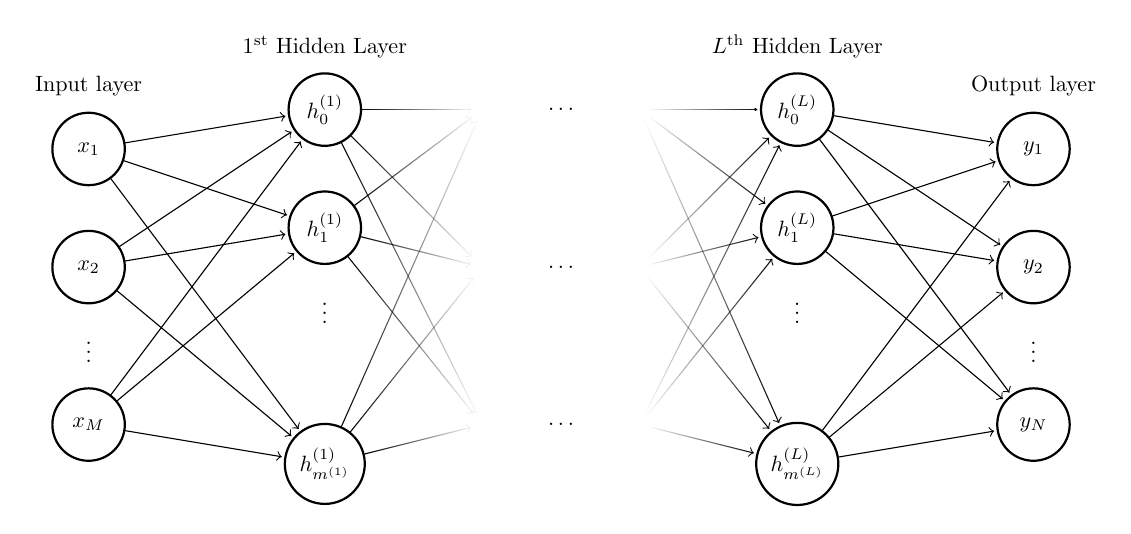
\begin{tikzpicture}[shorten >=1pt, every node/.style={scale=0.8, thick}]
		\tikzstyle{unit}=[draw,shape=circle,minimum size=1.15cm]
		\tikzstyle{hidden}=[draw,shape=circle,minimum size=1.15cm]
 
    % Input layer
		\node[unit](x0) at (0,3.5){$x_1$};
		\node[unit](x1) at (0,2){$x_2$};
		\node at (0,1){\vdots};
		\node[unit](xd) at (0,0){$x_M$};
 
    % 1st Hidden layer
		\node[hidden](h10) at (3,4){$h_0^{(1)}$};
		\node[hidden](h11) at (3,2.5){$h_1^{(1)}$};
		\node at (3,1.5){\vdots};
		\node[hidden](h1m) at (3,-0.5){$h_{m^{(1)}}^{(1)}$};
 
    % Hidden hidden layers
		\node(h20) at (5,4){};
		\node(h21) at (5,2){};
		\node(h22) at (5,0){};
		
		\node(d3) at (6,0){$\ldots$};
		\node(d2) at (6,2){$\ldots$};
		\node(d1) at (6,4){$\ldots$};
 
		\node(hL10) at (7,4){};
		\node(hL11) at (7,2){};
		\node(hL12) at (7,0){};
    
    % L'th hidden layer
		\node[hidden](hL0) at (9,4){$h_0^{(L)}$};
		\node[hidden](hL1) at (9,2.5){$h_1^{(L)}$};
		\node at (9,1.5){\vdots};
		\node[hidden](hLm) at (9,-0.5){$h_{m^{(L)}}^{(L)}$};
 
    % Output layer
		\node[unit](y1) at (12,3.5){$y_1$};
		\node[unit](y2) at (12,2){$y_2$};
		\node at (12,1){\vdots};	
		\node[unit](yc) at (12,0){$y_N$};
 
		\draw[->] (x0) -- (h10);
		\draw[->] (x0) -- (h11);
		\draw[->] (x0) -- (h1m);
 
		\draw[->] (x1) -- (h10);
		\draw[->] (x1) -- (h11);
		\draw[->] (x1) -- (h1m);
 
		\draw[->] (xd) -- (h10);
		\draw[->] (xd) -- (h11);
		\draw[->] (xd) -- (h1m);
 
		\draw[->] (hL0) -- (y1);
		\draw[->] (hL0) -- (y2);
		\draw[->] (hL0) -- (yc);
 
		\draw[->] (hL1) -- (y1);
		\draw[->] (hL1) -- (yc);
		\draw[->] (hL1) -- (y2);
 
		\draw[->] (hLm) -- (y1);
		\draw[->] (hLm) -- (y2);
		\draw[->] (hLm) -- (yc);
 
		\draw[->,path fading=east] (h10) -- (h20);
		\draw[->,path fading=east] (h10) -- (h21);
		\draw[->,path fading=east] (h10) -- (h22);
		
		\draw[->,path fading=east] (h11) -- (h20);
		\draw[->,path fading=east] (h11) -- (h21);
		\draw[->,path fading=east] (h11) -- (h22);
		
		\draw[->,path fading=east] (h1m) -- (h20);
		\draw[->,path fading=east] (h1m) -- (h21);
    	\draw[->,path fading=east] (h1m) -- (h22);

		\draw[->,path fading=west] (hL10) -- (hL0);
		\draw[->,path fading=west] (hL11) -- (hL0);
		\draw[->,path fading=west] (hL12) -- (hL0);
		
		\draw[->,path fading=west] (hL10) -- (hL1);
		\draw[->,path fading=west] (hL11) -- (hL1);
		\draw[->,path fading=west] (hL12) -- (hL1);
		
		\draw[->,path fading=west] (hL10) -- (hLm);
		\draw[->,path fading=west] (hL11) -- (hLm);
		\draw[->,path fading=west] (hL12) -- (hLm);
		
		\node[above of=x0, black]{Input layer};
		\node [above of=h10, black]{$1^{\text{st}}$ Hidden Layer};
		\node [above of=hL0, black]{$L^{\text{th}}$ Hidden Layer};
		\node[above of=y1, black]{Output layer};
  \end{tikzpicture}

\end{document}